\documentclass[10pt,twocolumn,letterpaper]{article}
\usepackage[review]{cvpr}
\usepackage{times,graphicx,amsmath,amssymb,booktabs,microtype,multirow}
\usepackage[accsupp]{axessibility}
\usepackage[pagebackref,breaklinks,colorlinks,allcolors=blue]{hyperref}
\def\paperID{-----}
\def\confName{CVPR}
\def\confYear{2027}
\newcommand{\R}{\mathbb{R}}
\newcommand{\norm}[1]{\left\lVert#1\right\rVert}
\title{Beyond Reconstruction: Decision and Temporal Fidelity\\in Graph-to-Spike Conversion}
\author{Anonymous authors}
\begin{document}
\maketitle
\begin{abstract}
Low-timestep conversion of graph neural networks is often assessed through activation or message reconstruction. What must such reconstruction preserve to retain a graph classifier's decision? We study this question by intervening on hard events in converted superpixel graph classifiers. Two gaps emerge. First, reducing the error of the actual graph message can worsen its downstream class margin: this occurs in 40.9\% and 31.9\% of message-improving interventions on MNIST and CIFAR10, respectively. Second, temporal codes with exactly the same local decoded output and event count can produce different downstream predictions and activity. A directional margin analysis and a source-recurrence counterexample explain why neither message magnitude nor terminal reconstruction determines decision fidelity. Three-teacher position interventions locate a major low-timestep bottleneck at the first node activation, while matched calibration controls distinguish this sensitivity from a realizable correction. Residual centering provides a constructive example of reducing a projection-activity proxy without resolving the decision problem. Together, these results identify the spatial direction and temporal history discarded by reconstruction metrics, and establish practical conditions for evaluating finite-event graph conversion.
\end{abstract}

\section{Introduction}
Graph neural networks make predictions by repeatedly mixing information over a graph. Converting their continuous representations to a small number of events changes both the values being propagated and the histories through which later layers receive them. For visual graphs, this coupling matters: an image-level decision can change when a perturbation at one superpixel crosses a downstream quantization boundary, even if an average reconstruction metric improves.

ANN-to-SNN conversion offers ways to approximate a pretrained network without retraining its weights. Calibration reduces activation mismatch, bias correction compensates temporal error, and differential coding represents changes rather than repeatedly transmitting rates~\cite{li2021,wu2024ftbc,huang2025}. These tools already support high-fidelity conversion at short prefixes. In our graph adaptations, four active ticks approximately preserve the accuracy of three independently trained teachers on both fixed and gated superpixel networks. Yet the shortest prefix behaves quite differently. This creates an informative regime in which to ask what reconstruction metrics retain, and what they leave out.

The distinction is sharper than an imperfect correlation between MSE and accuracy. A lower next-message error respects the actual adjacency and weights, but still discards the direction of that error relative to class boundaries. An exact local terminal reconstruction preserves even more information, yet discards intermediate states encountered by downstream event units. These are separate obstacles. A correction may improve the message norm while moving the final decision in the wrong direction; an alternative code may match its local output exactly while changing the downstream computation.

We investigate both obstacles using existing frozen graph classifiers and controlled hard-event interventions. The primary setting is MNIST and CIFAR10 superpixel classification with residual GCNs. A complementary GatedGCN study examines residual centering, and classical node classification provides historical context for propagation and readout effects. Throughout, we distinguish prediction agreement with the teacher from ground-truth accuracy, and local event counts from whole-network cost.

Our central finding is that \emph{reconstruction equivalence is weaker than decision equivalence in both space and time}. Hard, single-event changes provide direct evidence for the spatial gap. Among changes that reduce immediate message MSE, the teacher-class margin worsens in roughly one-third to two-fifths of cases. For the temporal gap, we construct two legal codewords with identical local two-tick decoding and show that exchanging them can change downstream predictions and activity on real graphs. These observations are supported by a three-teacher position analysis: recovering the first node activation closes 54.1\% and 23.5\% of the teacher-disagreement gap at one tick, whereas recovering both readout activations closes 8.8\% and 14.9\%.

The resulting contribution is an empirical and analytical account of the information a low-timestep conversion must preserve. We connect directional class margins to graph-propagated error, isolate temporal history with exact local equivalences, and evaluate calibration and representation controls under explicit budgets. This account explains why sensitivity, lower reconstruction error, and fewer local operations are useful diagnostics but different properties. It also yields a concrete evaluation rule: assess the decision and every required prefix after a realizable intervention, and measure the whole-network activity that follows it.

\begin{figure}[t]
\centering
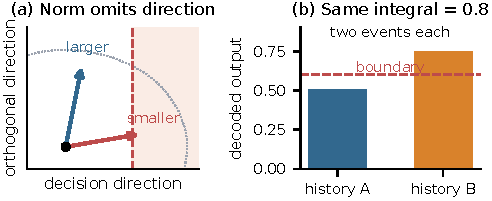
\includegraphics[width=\linewidth]{figures/concept.pdf}
\caption{Two information losses in reconstruction metrics. Left: a smaller error norm can cross a decision boundary when its direction changes (schematic). Right: two input histories have identical integrated input and two emitted events, but the fixed source neuron decodes them differently. The temporal values are an executable recurrence counterexample, rather than a dataset estimate.}
\label{fig:concept}
\end{figure}

\section{Related Work}
\paragraph{Conversion, calibration, and readout.}
Layerwise calibration adjusts converted networks using pretrained ANN responses~\cite{li2021}. Distribution-based threshold and potential initialization~\cite{bojkovic2024} and forward temporal bias correction~\cite{wu2024ftbc} address systematic approximation errors. These precedents make initial-potential fitting and bias compensation appropriate controls rather than independent algorithmic contributions here. Retaining a final membrane residual also preserves information discarded by integer spike counts. Our early node experiments use this distinction to separate hidden approximation from output quantization; we do not attribute it to a new neuron model.

Differential coding with graded units and spiking neurons (DCGS) transmits changes in represented activation and supplies a threshold-iteration procedure~\cite{huang2025}. We use its pinned public event unit in explicitly identified graph adaptations. One-Spike SNN already demonstrates GCN conversion~\cite{hwang2025onespike}; neither graph conversion itself nor an alternative temporal code establishes novelty. Temporal misalignment is also an established problem~\cite{bojkovic2025}. Our temporal experiment isolates a narrower issue: exact terminal equality at a local site need not preserve downstream decisions or total activity under the same finite event alphabet.

\paragraph{Graph-dependent approximation.}
Degree-Quant studies quantization-aware graph training, and A$^2$Q makes aggregation part of quantization design~\cite{degreequant2021,a2q2023}. These methods establish that graph structure matters to approximation. Our question concerns a frozen converted computation: does improving the actual immediate graph message preserve its final decision? Feature-only and permuted-operator controls test this question without changing the task graph or giving one policy extra fitting parameters. The visual models and data follow Benchmarking GNNs~\cite{dwivedi2023}. Results from static propagation, feature-dependent gating, and classical node classification are kept separate because they implement different operators and codes.

\section{Analysis and Experimental Design}
\subsection{Frozen graph computation and event semantics}
Our primary teacher has four residual graph-convolution layers of width 146. For fixed normalized adjacency $A$, its evaluation-mode layer is
\begin{equation}
 H_{\ell+1}=H_\ell+\operatorname{ReLU}(AH_\ell W_\ell^\top+b_\ell),
 \label{eq:block}
\end{equation}
with batch normalization folded into $W_\ell,b_\ell$. Node features and positions are embedded together. Mean pooling feeds a 146--73--36--10 MLP with two hidden ReLUs. The conversion has four node activation sites and two readout sites. Its graph operator weights each original directed edge $u\!\to\!v$ by $[\max(d_{\rm out}(u),1)\max(d_{\rm in}(v),1)]^{-1/2}$, without adding self-loops. The residual path supplies the identity connection.

An event is a signed scalar from $\{0,\pm\theta,\ldots,\pm\theta/128\}$, with per-channel threshold $\theta>0$. It is not a binary spike. Let $c_t$ be the current at active tick $t$, and let $(v,C,a,b)$ denote membrane, cumulative output, integrated input, and integrated output states. The source differential unit first computes
\begin{equation}
 m=v+c_t+a-b,\qquad \widetilde C=C+b.
\end{equation}
It emits the largest eligible magnitude $s_t$. A positive level $q=\theta2^{-k}$ requires $m\geq0.75q$; a negative level requires $m\leq-0.75q$ and $\widetilde C\geq q$. The updates are
\begin{equation}
\begin{split}
 v&\leftarrow m-s_t,\quad C\leftarrow\widetilde C+s_t,\\
 a&\leftarrow a+c_t/t,\quad b\leftarrow b+s_t/t.
\end{split}\label{eq:state}
\end{equation}
The decoder is $D_T(s)=\sum_{t=1}^T s_t/t$. Raw inputs and affine biases enter once, at the first active tick. We use $T$ for active ticks, not measured latency. Residual and readout arithmetic remains continuous where specified by the adapter.

\subsection{What a graph message norm does not determine}
For an activation perturbation $E$ at a fixed site, the immediate next-message perturbation is exactly
\begin{equation}
 \Delta M=AEW^\top.\label{eq:message}
\end{equation}
Consequently, $\norm{\Delta M}_F^2$ accounts for the actual propagation operator, but compresses a signed, graph-dependent perturbation to one scalar. A two-layer classifier with linear graph readout $R$ gives the particularly transparent relation $\Delta z=RAEW^\top$. This identity is elementary linear algebra. Its value here is to expose which information a norm omits.

Let $y=\arg\max_k z_k$ be the teacher class, and define its margin against every competitor $k\ne y$ by $m_k=z_y-z_k$. The converted prediction agrees with $y$ precisely when
\begin{equation}
 m_k+\Delta z_y-\Delta z_k>0\quad\text{for all }k\ne y,
 \label{eq:margin}
\end{equation}
apart from ties. In a linear downstream region, write $\Delta z=J\operatorname{vec}(E)$, with $J$ including the graph and readout. Then the relevant perturbations are the signed projections
\begin{equation}
 (J_y-J_k)\operatorname{vec}(E),
\end{equation}
rather than the reconstruction norm alone. A sufficient condition is
\begin{equation}
 \norm{\operatorname{vec}(E)}_2<
 \min_{k\ne y}\frac{m_k}{\norm{J_y-J_k}_2},\label{eq:sufficient}
\end{equation}
with zero rows imposing no restriction. Smaller norms tighten this worst-case bound; they do not order two actual errors pointing in different directions. In the full converted network, later event boundaries can also change $J$ or invalidate a fixed-region linearization. We therefore use Eq.~\eqref{eq:margin} as an exact decision condition and test message interventions with the actual hard forward pass.

For reported interventions, the scalar teacher-class margin is the converted logit of $y$ minus the largest converted competing logit. The competing class can change after intervention. Fixing the teacher's original runner-up can miss a newly dominant class. Ground-truth accuracy answers a different question: a converted prediction can disagree with an incorrect teacher and become correct. We retain both metrics instead of treating improved accuracy as evidence of improved conversion fidelity.

This perspective connects to early node-conversion analysis. Under nonsaturating constant-drive IF coding, rate error scales with $\theta/T$; retaining the membrane residual removes the final count quantization. Combining a valid hidden-error envelope with Eq.~\eqref{eq:sufficient} gives a sufficient time budget depending on propagation and margin. It does not imply that a common time budget, global bias sign, or row-stochastic bound applies to every graph. Symmetric degree normalization is not generally row stochastic. The supplementary material gives the readout identity, assumptions, and historical node results.

\subsection{What terminal reconstruction does not determine}
Equation~\eqref{eq:state} stores more than a decoded terminal activation. Replacing a first-tick event by $s_1+\delta$ must also change $v\leftarrow v-\delta$, $C\leftarrow C+\delta$, and $b\leftarrow b+\delta$. A later event consequently depends on both the incoming history and state. Matching $D_T(s)$ at one site cannot by itself match the intermediate currents received at its consumers.

A scalar counterexample uses exactly the frozen source recurrence, $\theta=1$, zero initial state, and $T=2$. The input histories $(c_1,c_2)=(0.01,1.58)$ and $(1,-0.4)$ have the same integrated input $c_1+c_2/2=0.8$. Both emit two nonzero events. Yet the decoded outputs are $0.5078125$ and $0.75$. A fixed decision boundary at $0.6$ separates them (Fig.~\ref{fig:concept}). Thus equality of integrated input, alphabet, time budget, and event count does not determine a nonlinear consumer's decoded result.

To test the same issue inside real graphs, we use source-verified first-site codeword pairs
\begin{equation}
 (q,-q/2)\quad\longleftrightarrow\quad(q/2,q/2).
 \label{eq:words}
\end{equation}
Both decode to $3q/4$ and contain two events (Fig.~\ref{fig:temporal-mechanism}). They differ at the first prefix and in unweighted absolute amplitude. We apply a replacement only when all levels belong to the original alphabet and actual source replay under the known zero second-tick input produces the required second event. Both directions are checked; the subsequent forward pass executes normally. This is an exact local equivalence test, not a proposed efficient encoder. Equality at every consumed tick, together with identical initial state, would preserve a deterministic downstream trajectory by induction. Equality only at its terminal tick is weaker. This is consistent with prior temporal-misalignment results~\cite{bojkovic2025}; our diagnostic isolates the ambiguity while enforcing exact local decoding and local event-count equality inside the graph adapter.

\begin{figure}[t]
\centering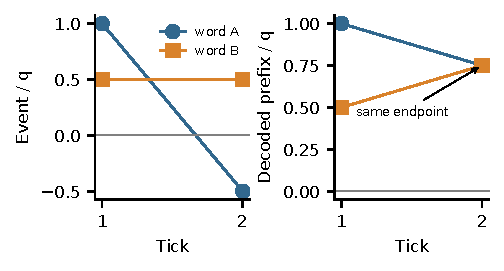
\includegraphics[width=\linewidth]{figures/temporal_mechanism.pdf}
\caption{The local equivalence test. Two legal codewords have two nonzero events and the same decoded endpoint $3q/4$, but present different first-prefix values to downstream consumers. Source replay verifies eligibility before replacement; the rest of the network is then executed without resetting its states.}
\label{fig:temporal-mechanism}
\end{figure}

\subsection{Interventions, controls, and evidence scope}
We use three complementary evidence levels. First, full historical official test predictions from three teacher seeds characterize conversion fidelity, and full validation position interventions localize error. Second, single-teacher hard interventions and calibration comparisons use 512 fixed, previously exposed validation graphs per task. Third, exact temporal-code tests use 128 training graphs per task, and the centered-residual profiles use all 45,000 CIFAR10 training graphs for one GatedGCN teacher. These splits serve different purposes. Official validation and test sets were exposed during earlier development; their results are descriptive evidence, not new blind confirmation.

For position analysis, an ideal causal ReLU replaces one selected converted activation while leaving the graph, weights, and incoming converted computation fixed. It is a continuous diagnostic. Restoring all six sites reproduces the ANN; an empty intervention reproduces the conversion. Group effects are nonadditive because interventions alter subsequent computation.

For hard intervention, we modify one existing nonzero first-site event up or down one legal amplitude level, update all affected states, and replay the network. Two label-free coordinate rules are used: a deterministic coordinate and the largest eligible local residual. The eligible coordinate sets can differ between upward and downward moves. Each task yields four attempts per graph, or 2,048 first-tick interventions. The teacher is used only afterward to measure margin and agreement. Confidence intervals resample graphs, retaining their repeated interventions together.

Calibration controls share teacher weights, histogram thresholds, 512 training graphs, 693 initial-potential offsets, and 64 Adam updates. The offsets are $\theta\rho$ with $\rho\in[-0.5,0.5]$. Local fitting averages normalized site MSE; graph-output fitting targets teacher logits; their mixture uses both. A second control family fits an immediate-message objective and compares actual $A$ with identity and within-graph conjugation $P^{-1}AP$. The graph used for the task is unchanged. We also retain the source 100-step threshold iteration and fallback rules as a graph adaptation; its placement, eight-level setting, and calibration horizon are specified separately in the supplement.

\section{Results}
\subsection{High fidelity and a concentrated short-prefix bottleneck}
Table~\ref{tab:main} establishes the operating regime. At four or eight ticks, the adapted differential code closely matches the teacher accuracy on both fixed GCNs and the stronger CIFAR10 GatedGCN. The latter retains continuous gates, products, normalization, and readout. Its high fidelity therefore demonstrates a hybrid graph adaptation, with different event placement from the fixed-GCN experiment.

\begin{table}[t]
\caption{Historical full-test accuracy (\%), mean $\pm$ sample SD over three teacher seeds on the same 10,000 graphs. The tests were previously exposed. GatedGCN is a separate hybrid adapter with continuous gates; the table establishes fidelity, not superiority of a new method.}
\label{tab:main}
\centering\small
\setlength{\tabcolsep}{3.5pt}
\begin{tabular}{lrrr}\toprule
Task / teacher & ANN & $T=4$ & $T=8$\\\midrule
MNIST / GCN & $91.02\pm.27$ & $91.05\pm.26$ & $91.02\pm.26$\\
CIFAR10 / GCN & $54.94\pm.07$ & $54.92\pm.08$ & $54.97\pm.05$\\
CIFAR10 / Gated & $68.77\pm.41$ & $68.75\pm.33$ & $68.76\pm.39$\\\bottomrule
\end{tabular}
\end{table}

At one tick, fixed-GCN conversion falls to $71.44\pm2.80\%$ on MNIST and $46.80\pm1.22\%$ on CIFAR10. Which sites cause this gap? Figure~\ref{fig:positions} shows conditional recovery on the full 5,000-graph validation split for each teacher. The first node site closes 54.08\% and 23.54\% of the disagreement gap, measured per teacher and then averaged. Recovering all four node sites closes 80.4\% and 45.2\%; the two readout sites close 8.8\% and 14.9\%. The first site is the largest single-site accuracy recovery on both tasks. This locates a useful intervention point, but the recovery uses a continuous response and imposes no finite-event constraint.

\begin{figure}[t]
\centering
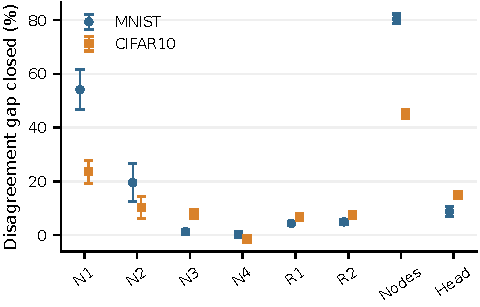
\includegraphics[width=\linewidth]{figures/position_recovery.pdf}
\caption{Conditional recovery at $T=1$ on full, previously exposed validation data. Gap closure is the recovered fraction of teacher disagreement, averaged across three teachers. Bars show sample SD across teachers. Node and readout groups restore four and two sites, respectively; effects cannot be added.}
\label{fig:positions}
\end{figure}

Classical node classification provides a compatible but distinct observation. Audited historical two-layer IF experiments approach their own ANN teachers at longer horizons when analytic bias compensation and membrane readout are used. For example, Cora reaches 80.16\% at $T=8$ against an 80.46\% teacher. The decoder and time scale differ from Table~\ref{tab:main}; supplementary results retain this separation rather than pooling the two as one converter.

\subsection{A better message can have a worse decision direction}
The controlled event changes directly test whether message improvement orders downstream decision quality. On MNIST, 811 of 2,048 interventions reduce the actual first-tick next-message MSE. Of these, 332 worsen the teacher-class margin: 40.94\%, with a graph-cluster bootstrap 95\% interval of [37.28,44.57]\%. On CIFAR10, the corresponding count is 296 of 928, or 31.90\% [28.66,35.31]\%. The same first-tick modifications worsen the $T=2$ margin in 48.71\% and 44.07\% of message-improving cases. These later percentages concern the same first-tick message metric, not cumulative two-tick message error.

\begin{figure}[t]
\centering
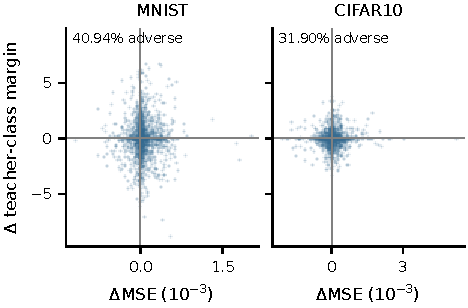
\includegraphics[width=\linewidth]{figures/message_decision.pdf}
\caption{Hard-event message improvement does not order decision improvement. Each point is a first-site intervention; horizontal change is immediate message MSE and vertical change is the teacher-class margin. The upper-left/lower-left split separates favorable/adverse margin changes among message improvements. All four attempts from each graph remain together for uncertainty estimation. Teacher 41, exposed validation; counts summarize $T=1$.}
\label{fig:mismatch}
\end{figure}

\begin{table}[t]
\caption{Core hard-intervention result. Among changes lowering first-tick message MSE, how often does the final teacher-class margin worsen? Each task has 512 graphs and 2,048 attempts. $T=2$ reuses the same interventions and MSE condition. Intervals are 95\% graph-cluster bootstrap.}
\label{tab:hard}\centering\small\setlength{\tabcolsep}{3pt}
\begin{tabular}{llrl}\toprule
Task & Readout & Adverse / improved & Rate [interval] (\%)\\\midrule
MNIST & $T=1$ & 332 / 811 & 40.94 [37.28,44.57]\\
 & $T=2$ & 395 / 811 & 48.71 [45.02,52.42]\\
CIFAR10 & $T=1$ & 296 / 928 & 31.90 [28.66,35.31]\\
 & $T=2$ & 409 / 928 & 44.07 [40.54,47.60]\\\bottomrule
\end{tabular}\end{table}

This is not confined to teachers with a small top-two margin. On MNIST validation graph 437, the teacher and ground truth are class 5, and the teacher's top-two margin is 5.20378. A deterministic downward event change reduces message MSE from 0.00604723 to 0.00604511, while the converted teacher-class margin changes from 1.97242 to $-3.74764$, flipping its prediction from 5 to 4. The message norm improves, but Eq.~\eqref{eq:margin} fails for the perturbed decision.

The same mismatch appears in finite residual allocation. Relative to local allocation, actual-message allocation reduces normalized message MSE from 0.001378 to 0.001280 on MNIST and from 0.002018 to 0.001717 on CIFAR10. However, on CIFAR10, 491 of 512 graphs improve this metric and 27 of those change from correct to incorrect. On MNIST the corresponding counts are 440 and 17. Gains elsewhere can offset these losses in aggregate accuracy; the important observation is that per-graph reconstruction improvement is not a monotone decision criterion. These policies share extra event opportunities, rather than exactly equal realized event counts.

\subsection{Sensitivity does not select a superior calibration target}
Table~\ref{tab:calibration} compares objectives under the same fitting resources. Local calibration already recovers much of the one-tick accuracy gap. Switching to graph-output or mixed fitting produces small, setting-dependent changes: output-minus-local differences on full historical tests are $+0.20/+0.18$ percentage points at MNIST $T=1/2$, and $-0.18/+0.19$ on CIFAR10. Full-validation differences are $-0.10/-0.13$ and $-0.27/+0.43$. A metric closer to the output does not automatically yield a more effective finite, surrogate-optimized correction.

\begin{table}[t]
\caption{Matched calibration on historical full tests. Accuracy (\%), mean $\pm$ sample SD across three teachers. All fitted objectives share 693 offsets, 512 training graphs, and 64 updates. Each historical horizon was calibrated separately; this is not the shared-prefix experiment below.}
\label{tab:calibration}
\centering\small\setlength{\tabcolsep}{3pt}
\begin{tabular}{llrrr}\toprule
Task & $T$ & Local & Output & Mixed\\\midrule
MNIST & 1 & $78.50\pm2.10$ & $78.70\pm2.19$ & $78.95\pm2.08$\\
 & 2 & $90.08\pm.26$ & $90.26\pm.35$ & $90.19\pm.44$\\
CIFAR10 & 1 & $49.92\pm.14$ & $49.75\pm.68$ & $49.72\pm.32$\\
 & 2 & $54.18\pm.14$ & $54.37\pm.26$ & $54.42\pm.25$\\\bottomrule
\end{tabular}
\end{table}

The single-teacher shared-prefix controls are also informative. Fitting logits at $T=1,2$ raises $T=1$ accuracy by 1.17 points relative to strong local fitting on each task, but CIFAR10 teacher agreement falls by 2.15 points. Their paired graph-sampling intervals for accuracy differences include zero. A top-two ranking objective decreases its hard training loss yet moves predictions toward previously unconstrained third classes: the fraction outside the teacher's top two rises from 4.69\% to 22.95\% on MNIST and from 9.47\% to 27.34\% on CIFAR10. Protecting one competitor leaves others in Eq.~\eqref{eq:margin} unprotected. These controls identify distinct limitations of proxy choice; they do not establish the optimality of the chosen optimizer or rule out other task-aware objectives.

The source threshold-iteration control provides a different correction mechanism. Calling its original moment estimates, 100 update steps and fallback rules yields one-tick accuracies of 71.48\%/45.31\% on MNIST/CIFAR10 with calibration horizon one. At four ticks, the same fitted thresholds yield 91.21\%/54.88\%. This comparison establishes that high-prefix fidelity and a severe first-prefix gap coexist under an alternative source-linked calibration, beyond the histogram preset. Its graph placement and eight-level configuration are adaptations; the results do not evaluate the original complete source converter on its published benchmarks.

\paragraph{Does graph structure add a decision signal?}
The actual-message objective uses the task operator, whereas the feature-only control omits propagation and the conjugated control relabels it relative to features. Actual-message allocation is close to conjugated allocation on MNIST ($79.49\%$ versus $79.30\%$), and equal to feature-only allocation on CIFAR10 ($49.22\%$). These controls weaken an attribution of aggregate gains specifically to using the correct adjacency. They are especially necessary on superpixel graphs: outdegree is fixed by construction, so outdegree variance cannot explain graph-to-graph changes. Reconstructed indegree and neighborhood variables do vary, but adding them after teacher margin gives small in-sample incremental $R^2$ values (0.004--0.035 across tasks and prefixes). This is a descriptive association, rather than independent prediction evidence.

\subsection{Identical local decoding can change the downstream network}
Figure~\ref{fig:temporal} tests Eq.~\eqref{eq:words} on the first 128 fixed training graphs of each task. Source replay and actual forwarding verify bitwise equality of the first-site $T=2$ decoded tensor, and exactly equal first-site nonzero event counts. Thus subsequent differences cannot be attributed to a changed local terminal representation or extra local events.

\begin{figure}[t]
\centering
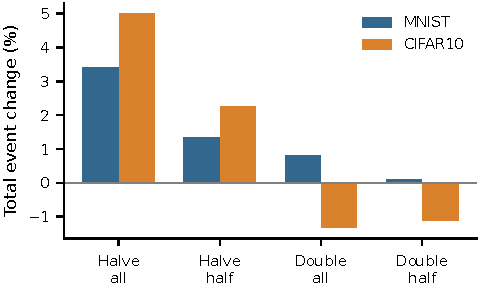
\includegraphics[width=\linewidth]{figures/temporal_equivalence.pdf}
\caption{Exact first-site $T=2$ equivalence does not preserve whole-network activity. Percentage change in total nonzero events after replacing all or a deterministic half of eligible codewords in either direction. The local decoded tensor and local two-tick event count are unchanged. Training-only diagnostic, 128 graphs per task; different directions have different eligible sets.}
\label{fig:temporal}
\end{figure}

When all eligible first events are halved, total $T=2$ events increase from 4,351,056 to 4,499,463 on MNIST and from 6,876,233 to 7,219,258 on CIFAR10. CIFAR10 accuracy changes from 66.41\% to 67.97\%, while teacher agreement falls from 85.16\% to 84.38\%. Reversing the exchange reduces CIFAR10 total events to 6,785,108 but gives different agreement again. On MNIST, reversing a deterministic half of eligible words changes $T=2$ accuracy from 94.53\% to 92.19\%. These are descriptive training-set effects, with no policy selected on their labels.

The exchange changes the first-prefix signal received by later layers. Their nonlinear event states integrate that signal before local equality is restored. A terminal hidden tensor is therefore not a sufficient summary of the downstream temporal computation. Likewise, reducing the first site's absolute event amplitude does not determine total events, amplitude, or graph delivery activity. The scalar counterexample isolates this state dependence; the graph experiment demonstrates its consequence in the actual residual network.

\subsection{Residual centering: a useful representation change with a limited guarantee}
A complementary GatedGCN diagnostic asks which part of a residual state needs event encoding. Write $h_\ell=h_0+q_\ell$ and $e_\ell=e_0+r_\ell$, where $q_\ell,r_\ell$ accumulate nonnegative residual branch increments. For a projection,
\begin{equation}
 Wh_\ell+b=(Wh_0+b)+Wq_\ell.\label{eq:center}
\end{equation}
The static carrier can be cached, and one encoded residual stream can serve the node consumers within a layer. Both compared implementations keep the first layer exact and preserve the same raw residual skip. Centering changes subsequent coded inputs from raw states to residual increments. Equation~\eqref{eq:center} is an affine identity; caching and shared streams are implementation opportunities, not new algebra.

\begin{figure}[t]
\centering
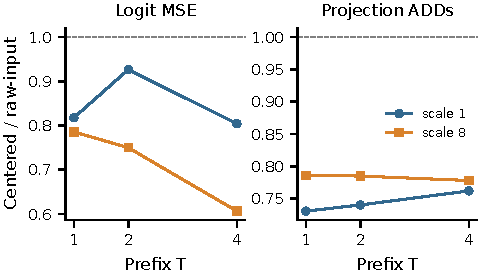
\includegraphics[width=\linewidth]{figures/centered_tradeoff.pdf}
\caption{Centered residual inputs relative to raw inputs after an identical exact first layer. All points use shared channel thresholds at a given scale. Ratios below one favor centered coding. Full 45,000-graph CIFAR10 training split, one GatedGCN teacher. ADDs count prospective coded projections only; they exclude static carriers and the rest of inference.}
\label{fig:centered}
\end{figure}

Under identical shared thresholds, centering lowers logit MSE and prospective coded-projection additions at every tested prefix ($T=1,2,4$) for both threshold scales (1 and 8). At scale 1 and $T=1$, teacher agreement rises by 2.04 points, while projected additions fall from $9.099\times10^{11}$ to $6.650\times10^{11}$ across the full training split. Agreement improves in five of six comparisons, with a 0.0044-point decrease at scale 1, $T=4$. This is constructive evidence that choosing the encoded origin matters even with matched thresholds. It measures teacher fidelity and one arithmetic component for one training-split teacher, rather than test accuracy or total runtime. It also exemplifies the central distinction: a favorable representation and local work proxy still require separate decision and complete-cost validation.

\subsection{Activity, simulation time, and applicability}
The primary conversion runs dense graph projections on every tick; zero events do not skip kernels. On an RTX 3060, synchronized cached-batch timings average 0.152/0.157 ms per graph for the MNIST/CIFAR10 ANN, versus 0.366/0.493 at $T=1$ and 1.238/1.762 at $T=4$ for the diagnostic converter. These are averages of three seed-level medians, using 32-graph batches and 30 interleaved repeats. They include decoded-site accumulation, exclude transfer and loading, and are not optimized deployment bounds. No chip energy is measured.

The distinction also matters for event allocation. Actual-message allocation costs 0.834/0.991 ms per graph versus local allocation's 0.668/0.806 in its own matched timing experiment. Exact local codeword exchanges can change downstream events even when first-site counts are fixed. Thus neither low $T$, local sparsity, nor the projected additions in Fig.~\ref{fig:centered} is a complete efficiency claim. A useful conversion must specify its event type, continuous work, prefix requirements, and backend.

\section{Discussion and Conclusion}
Our experiments identify two ways in which reconstruction metrics discard information needed for low-timestep graph decisions. A message norm discards direction relative to every competing class, and a terminal reconstruction discards the temporal states through which downstream units evolved. Position recovery shows where an intervention can matter; hard changes establish that a favorable local metric need not improve the decision; exact codeword exchanges reveal the remaining temporal ambiguity even after local terminal error is eliminated.

These observations suggest a disciplined design criterion. First determine which downstream quantity an approximation actually preserves. Then test a realizable finite-event change with fixed task computation, measure agreement and accuracy separately, and verify every required prefix together with total activity. Residual centering satisfies a useful representation identity and lowers a projection proxy, while task-aware calibration can change decisions without a consistent advantage. Their guarantees should be evaluated at the level they address.

The empirical scope is superpixel classification on fixed residual GCNs, supplemented by hybrid GatedGCN representation diagnostics and historical node experiments. The hard-event and temporal tests concern one teacher and previously used validation or training graphs. Independent task replication, direct One-Spike comparisons, and a modulewise decomposition of residual and event-boundary effects remain substantive extensions. Feature-dependent GatedGCN gates require their own perturbation analysis; changing input topology is outside the experiments. Within this scope, the evidence demonstrates that spatial message fidelity and local temporal equality are distinct from preserving the final graph decision. Making that distinction explicit is essential to interpreting low-timestep graph conversion.

\clearpage
\section*{LLM Usage Statement}
OpenAI Codex was used extensively for research-asset inspection, analysis and experimental code, evidence checks, mathematical discussion, manuscript organization and drafting, figure-generation code, and compilation checks. The final preparation used a GPT-6 based primary assistant and GPT-6-Luna assistants for bounded evidence and citation audits and data preparation. Earlier project stages used WorkBuddy for research planning and execution assistance, and Claude and Grok for written reviews and suggestions. Available historical records do not identify every underlying model version. The scientific results reported here originate from recorded numerical experiments and executable analyses; language-model suggestions are not treated as experimental evidence. The figures in this manuscript are programmatically rendered from recorded data or explicitly labeled mathematical examples, without generated experimental imagery. Human authors remain responsible for verifying all claims, citations, code, and disclosures and for approving any submission.

{\small
\bibliographystyle{ieeenat_fullname}
\bibliography{references}}
\end{document}
